\section{Background}\label{sec:introduction}

A chemist who wants a model for a molecular property usually starts with a table: one row per compound, a SMILES string, and a measured value. Turning that table into a trustworthy prediction involves three decisions that are made before any model is fitted. The first is whether the data can carry the weight placed on them: are the structures valid, are they duplicated, do the labels agree, and does the training set cover the chemistry that will be predicted \cite{fourches2010trust}? The second is which of several hundred computed descriptors \cite{todeschini2009descriptors,moriwaki2018mordred} should enter the model, if any. The third is the role those descriptors should play: passed to the model as additional input, used as a fixed baseline, or used as the starting point that a graph network corrects.

In practice these three decisions are encoded in task-specific scripts. The script mixes the chemical judgement with the engineering plumbing, so a reader cannot tell which options were tested, which were assumed, and which produced the reported number. Six months later the comparison is hard to repeat exactly. The problem is not a lack of algorithms. Descriptor-based models, fingerprints, and graph neural networks \cite{gilmer2017mpnn,yang2019dmpnn,xu2019gin} are all well developed, and benchmark collections such as MoleculeNet \cite{wu2018moleculenet} and the Therapeutics Data Commons \cite{huang2021tdc} allow systematic comparisons across endpoints \cite{mayr2018largescale,jiang2021gnn,deng2023systematic}. Prior work shows that descriptor-based models can match or outperform graph models on some tasks, and that adding descriptors to a learned graph representation can help on others \cite{aouichaoui2023gcgnn,wieder2020review}. The recurring lesson is that the usefulness of a representation depends on the endpoint, the curation of the data, and the evaluation protocol, not on the model class alone.

Decisions about features are equally consequential. Quantitative structure--activity and structure--property relationship (QSAR/QSPR) guidance asks for a defined endpoint, a transparent algorithm, and a stated applicability domain \cite{oecd2007guidance,tropsha2010best,cherkasov2014qsar}. Feature selectors address part of this: filters rank descriptors by correlation or mutual information \cite{guyon2003introduction,khan2018featureselection,shahlaei2013descriptor,danishuddin2016descriptors}, while embedded methods use a fitted learner, such as Random Forest importance \cite{strobl2007bias} or sparse regression, to rank them. Every such ranking is evidence for a particular dataset, learner, and budget. It is not a universal statement about which molecular properties matter, and presenting it as one is a common source of over-claiming.

A related decision is how the selected information enters the predictor. Descriptors may be concatenated with a learned graph representation, used as a fixed linear prior learned on the training set, or used as the baseline that the graph model corrects. We call the assignment of a feature block to a task a \emph{route}, and the way its output enters the predictor a \emph{role}. These roles answer different modelling questions, yet they are usually implemented in separate scripts or frozen into a pipeline, which makes an otherwise simple comparison expensive.

Open-source software already supplies much of the infrastructure. Chemprop provides efficient directed message-passing networks \cite{heid2024chemprop,graff2026chemprop}, DeepMol and QSARtuna automate pipeline and model search \cite{correia2024deepmol,mervin2024qsartuna,dixon2016autoqsar}, QSPRpred emphasises reproducible and serialisable QSPR workflows \cite{vandenmaagdenberg2024qsprpred}, ZairaChem targets automated screening cascades \cite{turon2023zairachem}, and integrated frameworks aim at scalable molecular property prediction \cite{chen2023integrated}. General tools such as Hydra and MLflow record settings and runs \cite{yadan2019hydra,zaharia2018mlflow}. The gap addressed here is narrower and, we argue, more useful to a chemist: none of these tools makes training-partition feature evidence, descriptor recommendations, feature routes, and predictive roles explicit inside one auditable experiment record (Table~\ref{tab:positioning}).

\begin{table}[t]
\caption{Emphasis of related open-source molecular machine-learning tools, summarised from the cited publications. Entries are not exhaustive feature lists.}
\label{tab:positioning}
\centering
\footnotesize
\setlength{\tabcolsep}{4pt}
\begin{tabular}{@{}>{\raggedright\arraybackslash}p{0.15\textwidth}>{\raggedright\arraybackslash}p{0.27\textwidth}>{\raggedright\arraybackslash}p{0.27\textwidth}>{\raggedright\arraybackslash}p{0.24\textwidth}@{}}
\toprule
Tool & Primary emphasis & Feature handling & Roles of feature groups \\
\midrule
Chemprop v2 \cite{graff2026chemprop} & Efficient, modular D-MPNN training and inference & Optional extra atom-, bond-, and molecule-level features & Direct (concatenated with the learned representation) \\
DeepMol \cite{correia2024deepmol} & Automated search over preprocessing, representation, and model pipelines & Feature extraction and selection as pipeline steps & Direct model input \\
QSARtuna \cite{mervin2024qsartuna} & Automated QSAR model and hyperparameter optimisation & Choice among descriptor and fingerprint representations & Direct model input \\
QSPRpred \cite{vandenmaagdenberg2024qsprpred} & Reproducible, serialisable QSPR modelling, including proteochemometrics & Training-only variance, correlation, and Boruta \cite{kursa2010boruta} filters & Direct model input \\
This work & Auditable link between feature evidence and model configuration & Training-partition evidence scorecard, dataset audit, relevance and redundancy recommender & Direct, fixed prior, or learned residual, declared per feature block \\
\bottomrule
\end{tabular}
\end{table}

We therefore built \framework, an open-source Python package in which an experiment is declared in one plain-text configuration file. The file names the dataset, the molecular representations, the split, the model, and the role of each descriptor block; it is checked against a typed schema before any computation starts. Fig.~\ref{fig:workflow} shows the five stages a user goes through, from a table of SMILES and measured values to a saved record that another person can replay. The framework does not replace the chemist's judgement. It makes each judgement visible, testable, and cheap to change.

\begin{figure}[t]
\centering
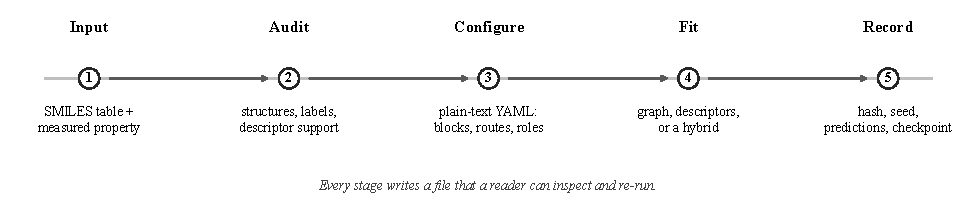
\includegraphics[width=0.98\textwidth]{figs/fig1_pipeline.pdf}
\caption{The five stages of a \framework{} experiment. A table of SMILES and measured properties is read and audited, the experiment is declared in a validated configuration file, the selected representations are fitted, and every run writes a record (configuration hash, split seed, predictions, checkpoint) that a reader can inspect and re-run. The framework changes what is explicit, not what is chemically possible.}
\label{fig:workflow}
\end{figure}

\subsection*{What this study tests}

The paper is organised around three hypotheses, stated here so that the reader can judge the results against them rather than after the fact.

\begin{description}\sloppy
\item[H1 --- Evidence is usable.] Training-partition diagnostics of descriptors, together with a transparent relevance-and-redundancy rule, carry enough information to guide descriptor choice. \emph{Prediction:} (i) descriptor subsets chosen from this evidence should beat random subsets of the same size in most dataset--budget cells tested; (ii) the rule should rank in the upper half of the selectors compared against it; and (iii) the choice should be stable across splits. \emph{Falsified if:} the evidence-based choice is indistinguishable from a random one, or if the rule ranks in the lower half of the selectors.
\item[H2 --- The descriptor effect transfers.] The effect of adding descriptors to a graph model is a property of the endpoint and the data, not of one software implementation. \emph{Prediction:} an independently written implementation (Chemprop v2.3.1, with a different encoder, featurisation and training loop) should change in the same direction and by a similar amount on most endpoints. Because the two systems differ in more than the descriptor block, agreement is evidence that the effect transfers, not a decomposition of it into architecture and features; the architecture-unconfounded estimate is the within-system contrast. \emph{Falsified if:} the two implementations disagree in sign across endpoints.
\item[H3 --- Route and role matter, but not universally.] Compact descriptor routes and alternative predictive roles change results, yet the best choice is endpoint-specific and small compared with split-to-split variation. \emph{Prediction:} no single route or role wins everywhere, and most differences should be comparable to the between-split standard deviation. \emph{Falsified if:} one configuration wins on every endpoint by a margin that exceeds the split variation.
\end{description}

Testing these hypotheses requires more than a new script. It requires the same splits, the same checkpoints, and the same evaluation rule across every model, and it requires that the comparison be reproducible by someone who did not run it. The remainder of the paper reports the design (Methods), the results for each hypothesis (Results), what they do and do not imply for a practising chemist (Discussion), and the conclusions (Conclusions). Table~\ref{tab:result-map} maps each hypothesis to its experiment and to the section and table where the evidence is reported.

\begin{table}[t]
\caption{Reading map: each hypothesis, the experiment that tests it, and where the answer is reported.}
\label{tab:result-map}
\centering
\footnotesize
\setlength{\tabcolsep}{4pt}
\begin{tabular}{@{}>{\raggedright\arraybackslash}p{0.05\textwidth}>{\raggedright\arraybackslash}p{0.26\textwidth}>{\raggedright\arraybackslash}p{0.36\textwidth}>{\raggedright\arraybackslash}p{0.23\textwidth}@{}}
\toprule
 & Hypothesis & Experiment & Reported in \\
\midrule
H1 & Training-partition evidence guides descriptor choice & Scorecard and dataset audit on five endpoints; six selectors at four budgets with a Random Forest downstream; recommended versus random subsets & Descriptor evidence and data audit; Tables~\ref{tab:selectors} and \ref{tab:hygiene}; Fig.~\ref{fig:worked} \\
H2 & The descriptor effect transfers between implementations & Graph-only and graph-plus-descriptor models in \framework{} and in Chemprop v2.3.1, on the same saved splits & Predictive performance; Tables~\ref{tab:baselines-regression} and \ref{tab:baselines-classification}; Fig.~\ref{fig:descriptor-effect} \\
H3 & Route and role matter, but the best choice is endpoint-specific & Five role configurations; a harmonised routing experiment with Spearman, mutual-information and random controls; per-split paired comparisons & Descriptor routing and predictive roles; Tables~\ref{tab:routing} and \ref{tab:ablation}; Fig.~\ref{fig:routing} \\
\bottomrule
\end{tabular}
\end{table}
